\chapter{Container Isolation}

In questa parte vedremo vari concetti che uniti insieme permetteranno di creare
un ambiente isolato che corrisponderà in utto e per tutto ad un container docker.

\section{Namespaces}

Se i cgroup controllano le risorse che un processo può utilizzare, allora i
\textit{namespace} controlla ciò che i processi possono vedere, dunque restringe
il numero di risorse visibili ad un dato processo.
La sua origine viene datata al sistemao operativo Plan 9 che fu il primo ad
introdurle ed usare.
Oggigiorno ci sono molti tipi di namespace supportati da linux:

\begin{itemize}
    \item Unix Timesharing System (UTS)
    \item Process IDs
    \item Mount Points
    \item Network
    \item User and group IDs
    \item Inter-process Communications (IPC)
    \item Cotrol Groups (cgroups)
\end{itemize}

Un processo è sempre esattamente in un namespace di ogni tipo.
Quando linux viene avviato ha un solo namespace per ogni tipo, ma come vedremo
a breve è possibile crearne di nuovi ad eggiungergli processi.\\

È possibile vedere tutti i namespace nella propria macchina con il comando
\verb|lsns|.

\begin{figure}[H]
    \centering
    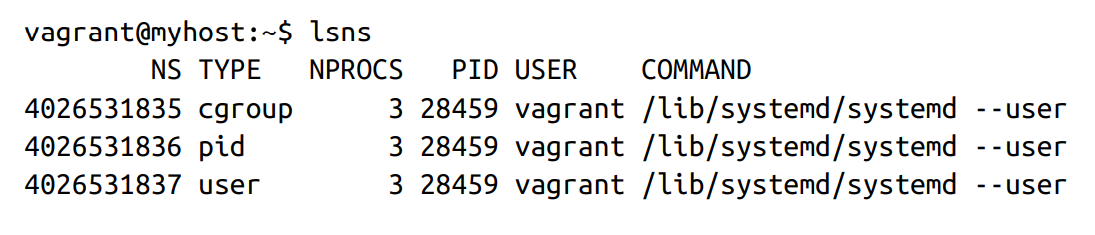
\includegraphics[width=\textwidth, keepaspectratio]{capitoli/os_security/imgs/namespace1.png}
\end{figure}

Eseguire il precedente comando senza i privilegi di root non fornisce tutta la lista
completa dei namesapce e dunque per vederli tutti sarà necessario esegruire il comando
con \verb|sudo|.

\begin{figure}[H]
    \centering
    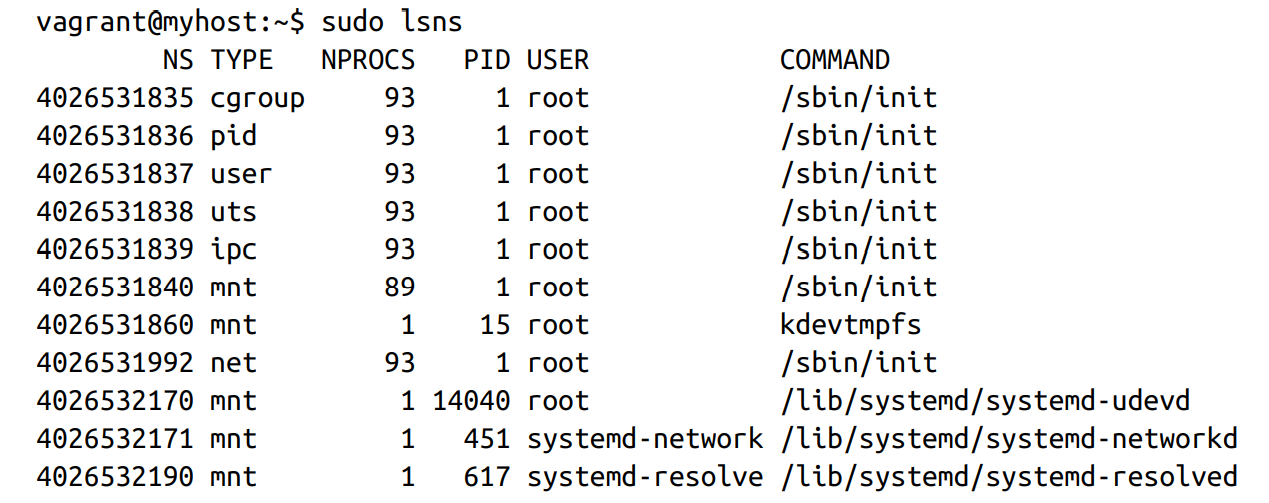
\includegraphics[width=\textwidth, keepaspectratio]{capitoli/os_security/imgs/namespace2.png}
\end{figure}

Vediamo ora come è possibile utilizzare i namespace per creare qualcosa che si
comporti come un container.

\section{Isolare l'Hostname}

Partiamo dal namespace UTS, questo permette di cambiare l'hostname di un processo
indipendentemente da quello della macchina (isola l'hostname).
Un esempio pratico di questo sono i container docker che hanno un proprio hostname
(generalmente l'ID che docker crea automaticamente ad ogni contianer) diverso da
quello del resto del sistema.

\begin{figure}[H]
    \centering
    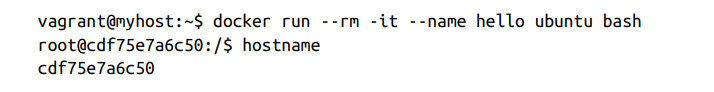
\includegraphics[width=\textwidth, keepaspectratio]{capitoli/os_security/imgs/hostname1.png}
\end{figure}

Docker riesce ad ottenere questo perchè crea il suo UTS namespace.
È possibile ottenre un comportamento simile con il comando \verb|unshare| e creare
un processo con il suo UTS namespace.\\

Il comando \verb|unshare| permette di "eseguire un programma con alcuni namespace
separati dal processo padre". Quando un programma viene lanciato, il kernel crea un
nuovo processo e ci esegue il codice del programma. Questa creazione parte dal
contesto di un processo, chiamato \textit{padre}, e
genera un nuovo processo chiamato \textit{figlio}. La parola "unshare" sta ad indicare
il fatot che invece che condividere il namespace del padre, il figlio ne avrà uno tutto suo.
Proviamo ad ottenere questo comportamento, avremmo bisogno dei permessi root,
quindi il comando andrà eseguito come \verb|sudo|.

\begin{figure}[H]
    \centering
    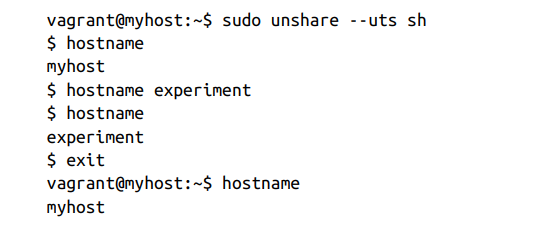
\includegraphics[width=10cm, keepaspectratio]{capitoli/os_security/imgs/hostname2.png}
\end{figure}

Il comando precedente avvia la shell \verb|sh| in un nuovo processo con il proprio
UTS namespace. Possiamo notare che cambiando l'hostname in questo processo
non va a modificare quello del resto del sistema. Se apriamo un altro terminale
prima del comando \verb|exit| possiamo notare come l'hostname non è stato
modificato. Grazie all'UTS namespace possiamo
cambiare l'hostname dell'host senza intaccare quello del processo e viceversa.\\

I namespace sono una compenente chiave del funzionamento dei container in quanto
permettono di assegnargli un set di risorse indipendenti dal resto del sistema host
e dagli altri container.

\section{Isolare i Process ID}

Vediamo ora come poter far vedere ad un container solo i processi che ha avviato e
non tutti quelli del sistema host.
In un container docker possiamo vedere solo i processi che girano al suo interno
senza avere accesso a tutti gli altri dell'host. Cerchiamo di raggiungere lo
stesso risultato. Possiamo usare ancora il comando \verb|unshare| specificando
che vogliamo un nuovo PID namesapce con il flag \verb|--pid|:


\begin{figure}[H]
    \centering
    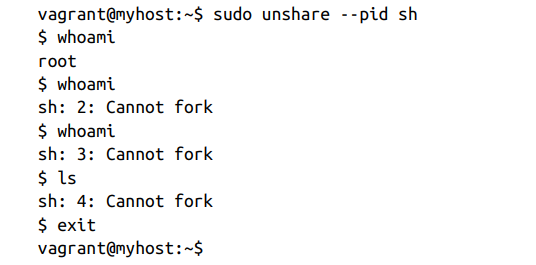
\includegraphics[width=10cm, keepaspectratio]{capitoli/os_security/imgs/pid1.png}
\end{figure}

Non sembra funzionare correttamente ma qualcosa ha fatto, analizziamolo.
Il primo comando sembra aver funzionato correttamente, ma dal secondo in poi
otteniamo un errore. Possiamo notare che gli errori sono formattati nel segunete modo:
\verb|<command>: <process ID>: <message>|. Dal secondo in poi notiamo che i PID
stanno incrementando e possiamo supporre che il PID del primo comando sia 1. Quindi
in un certo modo abbiamo ottenuto quello che volevamo.\\
Per risolvere questo problema ci viene in auito il manuale di \verb|unshare| che ci
suggerisce di utilizzare il flag \verb|--fork|: "effettua il fork del programma
specificato come processo figlio di unshare invece di eseguirlo direttamente".
Per come abbiamo eseguito il comando ora abbiamo la seguente situazione:

\begin{figure}[H]
    \centering
    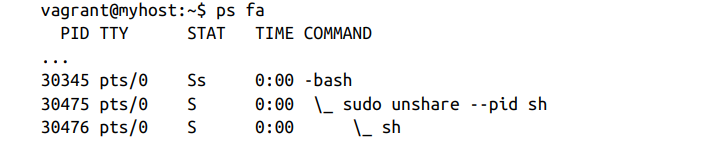
\includegraphics[width=12cm, keepaspectratio]{capitoli/os_security/imgs/pid2.png}
\end{figure}

Notiamo come il processo \verb|sh| non è figlio di \verb|unshare| ma del processo
\verb|sudo|.\\

Proviamo con il nuovo flag:

\begin{figure}[H]
    \centering
    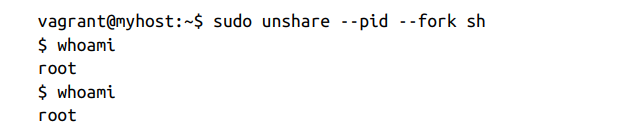
\includegraphics[width=12cm, keepaspectratio]{capitoli/os_security/imgs/pid3.png}
\end{figure}

Ora funziona correttamente. Possiamo eseguire più comandi in successione ed
analizzando la situazione attuale abbiamo:

\begin{figure}[H]
    \centering
    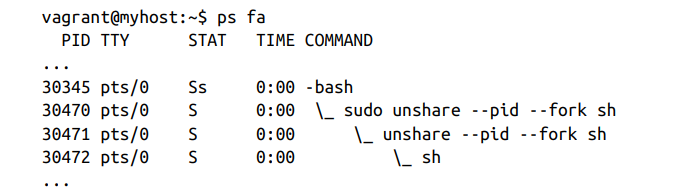
\includegraphics[width=12cm, keepaspectratio]{capitoli/os_security/imgs/pid4.png}
\end{figure}

Eseguendo il comando \verb|ps| all'interno del container ci accorgiamo che
possiamo comunque vedere tutti i processi dell'host anche se ci tronviamo
in un nuovo namespace.

\begin{figure}[H]
    \centering
    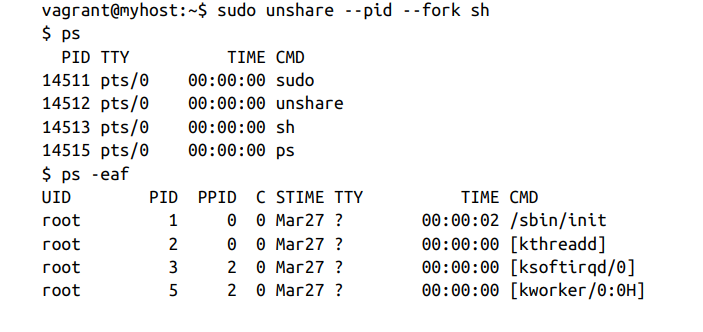
\includegraphics[width=12cm, keepaspectratio]{capitoli/os_security/imgs/pid5.png}
\end{figure}

Questo avviene perchè \verb|ps| legge i file virtuali contenuti nella cartella
\verb|/proc|. Andiamo a vedere ora il contenuto di questa directroy.

\begin{figure}[H]
    \centering
    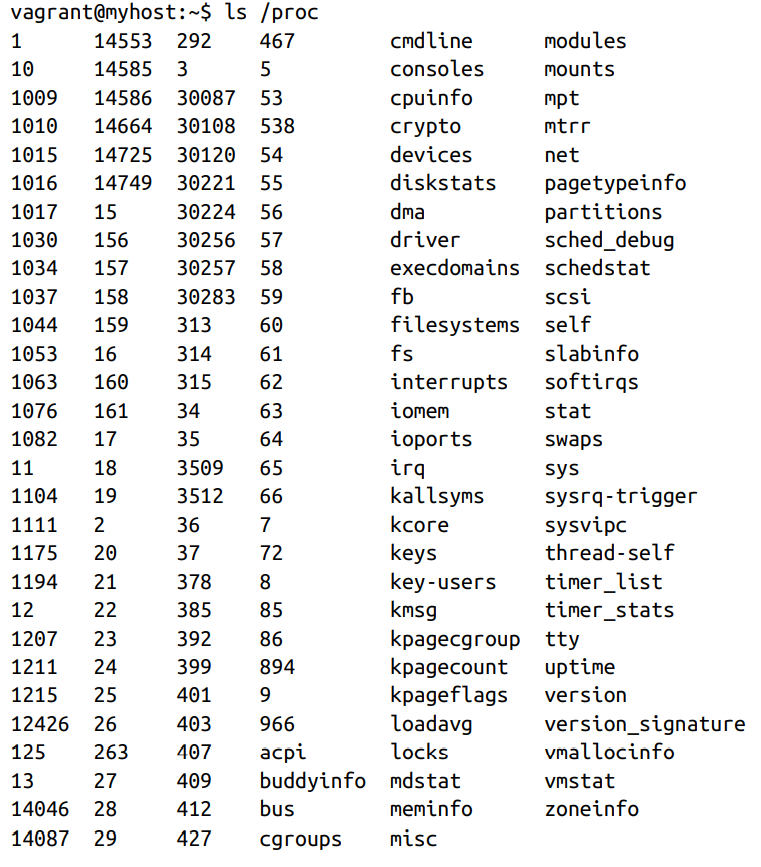
\includegraphics[width=12cm, keepaspectratio]{capitoli/os_security/imgs/pid6.png}
\end{figure}

Ogni directroy numerata all'interno di \verb|/proc| corrisponde ad un Process ID,
che contiene molte informazioni riguarante il processo. Per esempio il file
\verb|/proc/<pid>/exe| è un \textit{link simbolico} all'eseguibile del processo
con pid \verb|<pid>|.

\begin{figure}[H]
    \centering
    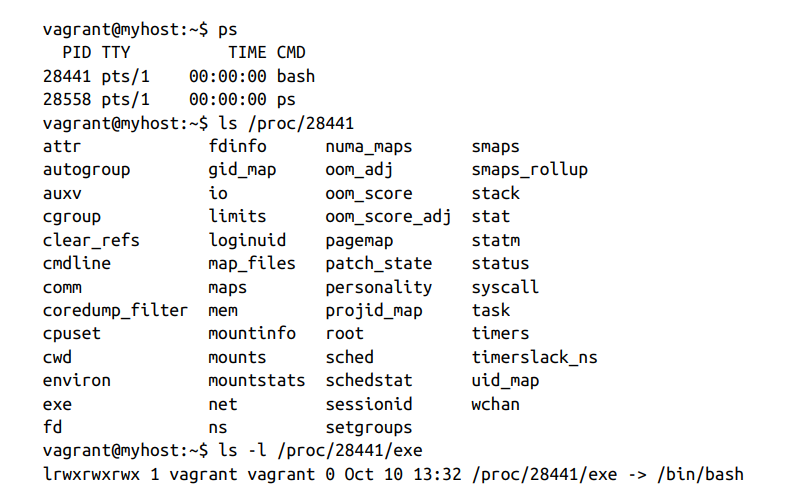
\includegraphics[width=12cm, keepaspectratio]{capitoli/os_security/imgs/pid7.png}
\end{figure}

Dunque per far si che \verb|ps| mostri solo i processi all'interno del nuovo
namespace servirà una copia della directroy \verb|/proc| in cui il kernel
potrà scrivere le informazioni riguardanti i nuovi processi e dato che
\verb|/proc| si trova sotto root, questo implica cambiare la directroy di root.

\section{Cambiare Root Directory}

La directroy di root può essere cambiata con il comando \verb|chroot| e
una volta effettuato questo comando si perde l'accesso ad ogni cosa che si trova
al di sopra della nuova directroy di root nella gerarchia del file system.

\begin{figure}[H]
    \centering
    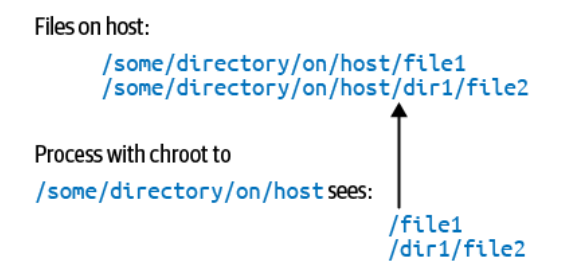
\includegraphics[width=10cm, keepaspectratio]{capitoli/os_security/imgs/root1.png}
\end{figure}

Va fatto notare che quando si va a cambiare la directroy di root si perdono anche
tutti gli eseguibili che sia hanno a disposizione solitamente in linux. Sarà
dunque necessario copiare questi file nella nuova directroy di root che è
quello che viene effettuato da docker quando istanzia l'immagine del container.

\begin{figure}[H]
    \centering
    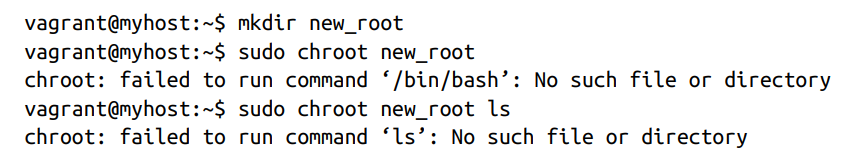
\includegraphics[width=\textwidth, keepaspectratio]{capitoli/os_security/imgs/root2.png}
\end{figure}

\section{Combinare Namespace con Chroot}

